\documentclass{article}\usepackage[]{graphicx}\usepackage[]{color}
%% maxwidth is the original width if it is less than linewidth
%% otherwise use linewidth (to make sure the graphics do not exceed the margin)
\makeatletter
\def\maxwidth{ %
  \ifdim\Gin@nat@width>\linewidth
    \linewidth
  \else
    \Gin@nat@width
  \fi
}
\makeatother

\definecolor{fgcolor}{rgb}{0.345, 0.345, 0.345}
\newcommand{\hlnum}[1]{\textcolor[rgb]{0.686,0.059,0.569}{#1}}%
\newcommand{\hlstr}[1]{\textcolor[rgb]{0.192,0.494,0.8}{#1}}%
\newcommand{\hlcom}[1]{\textcolor[rgb]{0.678,0.584,0.686}{\textit{#1}}}%
\newcommand{\hlopt}[1]{\textcolor[rgb]{0,0,0}{#1}}%
\newcommand{\hlstd}[1]{\textcolor[rgb]{0.345,0.345,0.345}{#1}}%
\newcommand{\hlkwa}[1]{\textcolor[rgb]{0.161,0.373,0.58}{\textbf{#1}}}%
\newcommand{\hlkwb}[1]{\textcolor[rgb]{0.69,0.353,0.396}{#1}}%
\newcommand{\hlkwc}[1]{\textcolor[rgb]{0.333,0.667,0.333}{#1}}%
\newcommand{\hlkwd}[1]{\textcolor[rgb]{0.737,0.353,0.396}{\textbf{#1}}}%
\let\hlipl\hlkwb

\usepackage{framed}
\makeatletter
\newenvironment{kframe}{%
 \def\at@end@of@kframe{}%
 \ifinner\ifhmode%
  \def\at@end@of@kframe{\end{minipage}}%
  \begin{minipage}{\columnwidth}%
 \fi\fi%
 \def\FrameCommand##1{\hskip\@totalleftmargin \hskip-\fboxsep
 \colorbox{shadecolor}{##1}\hskip-\fboxsep
     % There is no \\@totalrightmargin, so:
     \hskip-\linewidth \hskip-\@totalleftmargin \hskip\columnwidth}%
 \MakeFramed {\advance\hsize-\width
   \@totalleftmargin\z@ \linewidth\hsize
   \@setminipage}}%
 {\par\unskip\endMakeFramed%
 \at@end@of@kframe}
\makeatother

\definecolor{shadecolor}{rgb}{.97, .97, .97}
\definecolor{messagecolor}{rgb}{0, 0, 0}
\definecolor{warningcolor}{rgb}{1, 0, 1}
\definecolor{errorcolor}{rgb}{1, 0, 0}
\newenvironment{knitrout}{}{} % an empty environment to be redefined in TeX

\usepackage{alltt}
\IfFileExists{upquote.sty}{\usepackage{upquote}}{}
\begin{document}

\title{The Strange Case of Dr. Jekyll \& Mr. Hyde in Wordclouds}
\author{Elizabeth Bross}
\maketitle

\begin{abstract}

In this article we will construct two wordclouds, using the tidytext R package, for Robert Louis Stevenson's novel \textit{The Strange Case of Dr. Jekyll \& Mr. Hyde}. For those unfamiliar, \textit{The Strange Case of Dr. Jekyll \& Mr. Hyde} is a story set in Victorian era London about a series of odd coincidents bewtween two opposite characters: the kind Dr. Henry Jekyll and the evil Mr. Edward Hyde. As the story progresses, the reader becomes aware that Jekyll and Hyde are indeed the same person. The other characters are tasked with connecting occurances and eventually realize Dr. Jekyll transforms into Hyde by drinking a serum he invented. To capture the `good versus evil' theme of the book, we will create two wordclouds using opposing sentiment categories.

\end{abstract}

\section{The gutenbergr Package}
The package for R, gutenbergr, that gives one electronic access to over 50,000 free books. The collection is made up of the world's great titles from throughout history and includes older works with expired copyrights\footnote{you can find more information on Project Gutenberg here:  https://www.gutenberg.org/}. To begin this project, install the required packages and download the text. The gutenberg\_id number for \textit{The Strange Case of Dr. Jekyll \& Mr. Hyde} is 42. 

\begin{knitrout}
\definecolor{shadecolor}{rgb}{0.969, 0.969, 0.969}\color{fgcolor}\begin{kframe}
\begin{alltt}
\hlkwd{library}\hlstd{(tm)}
\hlkwd{library}\hlstd{(tidytext)}
\hlkwd{library}\hlstd{(dplyr)}
\hlkwd{library}\hlstd{(knitr)}
\hlkwd{library}\hlstd{(gutenbergr)}
\hlkwd{library}\hlstd{(stringr)}
\hlkwd{library}\hlstd{(wordcloud)}
\hlstd{JandH}\hlkwb{<-}\hlkwd{gutenberg_download}\hlstd{(}\hlnum{42}\hlstd{)}
\end{alltt}
\end{kframe}
\end{knitrout}

\section{Data Preparation}

We must first create a dataframe of all the words in the novel. This is easy to do with tidytext package. Use the unnest\_tokens function to break down the words into a dataframe.

\begin{knitrout}
\definecolor{shadecolor}{rgb}{0.969, 0.969, 0.969}\color{fgcolor}\begin{kframe}
\begin{alltt}
\hlstd{JandH_words}\hlkwb{<-}\hlstd{JandH}\hlopt
  \hlkwd{unnest_tokens}\hlstd{(word,text)}
\end{alltt}
\end{kframe}
\end{knitrout}

\noindent To determine which words we will look at, we will use those listed in the sentiment lexicon `nrc'. The tidytext package provides four sentiment lexicons. The `nrc' lexicon assign one of ten descriptions to important words in the English language. This technique eliminates the need to remove `stopwords'\footnote{a list of stopwords is available in the R package tm.} which are common, irrelevent words. 

\begin{knitrout}
\definecolor{shadecolor}{rgb}{0.969, 0.969, 0.969}\color{fgcolor}\begin{kframe}
\begin{alltt}
\hlstd{nrc}\hlkwb{<-}\hlkwd{get_sentiments}\hlstd{(}\hlstr{'nrc'}\hlstd{)}
\hlkwd{unique}\hlstd{(nrc}\hlopt{$}\hlstd{sentiment)}
\end{alltt}
\begin{verbatim}
##  [1] "trust"        "fear"         "negative"     "sadness"     
##  [5] "anger"        "surprise"     "positive"     "disgust"     
##  [9] "joy"          "anticipation"
\end{verbatim}
\begin{alltt}
\hlstd{nrc_fear}\hlkwb{<-}\hlstd{nrc}\hlopt
  \hlkwd{filter}\hlstd{(sentiment} \hlopt \hlkwd{c}\hlstd{(}\hlstr{'fear'}\hlstd{,}\hlstr{'negative'}\hlstd{,}
                          \hlstr{'sadness'}\hlstd{,}\hlstr{'anger'}\hlstd{,}\hlstr{'disgust'}\hlstd{))}

\hlstd{nrc_happy}\hlkwb{<-}\hlstd{nrc}\hlopt
  \hlkwd{filter}\hlstd{(sentiment} \hlopt \hlkwd{c}\hlstd{(}\hlstr{'trust'}\hlstd{,}\hlstr{'surprise'}\hlstd{,}
                          \hlstr{'positive'}\hlstd{,}\hlstr{'joy'}\hlstd{,}\hlstr{'anticipation'}\hlstd{))}
\end{alltt}
\end{kframe}
\end{knitrout}

\noindent Then, use the inner\_join function to match the words in our newly created dataframe JandH\_words with words provided in the nrc lexicon.

\begin{knitrout}
\definecolor{shadecolor}{rgb}{0.969, 0.969, 0.969}\color{fgcolor}\begin{kframe}
\begin{alltt}
\hlstd{JandH_fear_words}\hlkwb{<-}\hlkwd{inner_join}\hlstd{(nrc_fear,JandH_words)}
\hlstd{JandH_happy_words}\hlkwb{<-}\hlkwd{inner_join}\hlstd{(nrc_happy,JandH_words)}
\end{alltt}
\end{kframe}
\end{knitrout}

\section{The Wordclouds}

To begin creating the word coulds, use dplyr to calculate the frequency of words included in the JandH\_fear\_words dataframe. Be sure to create a new dataframe to make the creation of the final wordcloud easier.

\begin{knitrout}
\definecolor{shadecolor}{rgb}{0.969, 0.969, 0.969}\color{fgcolor}\begin{kframe}
\begin{alltt}
  \hlstd{JandH_fear_freq}\hlkwb{<-}\hlstd{JandH_fear_words}\hlopt
  \hlkwd{group_by}\hlstd{(word)}\hlopt
  \hlkwd{summarize}\hlstd{(}\hlkwc{count}\hlstd{=}\hlkwd{n}\hlstd{())}
\end{alltt}
\end{kframe}
\end{knitrout}

\noindent Then repeat this step on the JandH\_happy\_words dataframe.

\begin{knitrout}
\definecolor{shadecolor}{rgb}{0.969, 0.969, 0.969}\color{fgcolor}\begin{kframe}
\begin{alltt}
\hlstd{JandH_happy_freq}\hlkwb{<-}\hlstd{JandH_happy_words}\hlopt
  \hlkwd{group_by}\hlstd{(word)}\hlopt
  \hlkwd{summarize}\hlstd{(}\hlkwc{count}\hlstd{=}\hlkwd{n}\hlstd{())}
\end{alltt}
\end{kframe}
\end{knitrout}

\noindent Finally, use the wordcloud() function to create the fear themed wordcloud. In context of \textit{The Strange Case of Dr. Jekyll \& Mr. Hyde}, you could call this the Hyde wordcloud. Set the min.freq to 5 to avoid overloading your wordcloud.
\begin{knitrout}
\definecolor{shadecolor}{rgb}{0.969, 0.969, 0.969}\color{fgcolor}\begin{kframe}
\begin{alltt}
\hlkwd{wordcloud}\hlstd{(JandH_fear_freq}\hlopt{$}\hlstd{word,JandH_fear_freq}\hlopt{$}\hlstd{count,}\hlkwc{min.freq} \hlstd{=} \hlnum{5}\hlstd{)}
\end{alltt}
\end{kframe}

\includegraphics[width=\maxwidth]{figure/unnamed-chunk-7-1} 

\end{knitrout}

\noindent Repeat with JandH\_happy\_freq to create your Jekyll wordcloud.
\begin{knitrout}
\definecolor{shadecolor}{rgb}{0.969, 0.969, 0.969}\color{fgcolor}\begin{kframe}
\begin{alltt}
\hlkwd{wordcloud}\hlstd{(JandH_happy_freq}\hlopt{$}\hlstd{word,JandH_happy_freq}\hlopt{$}\hlstd{count,}\hlkwc{min.freq} \hlstd{=} \hlnum{5}\hlstd{)}
\end{alltt}
\end{kframe}
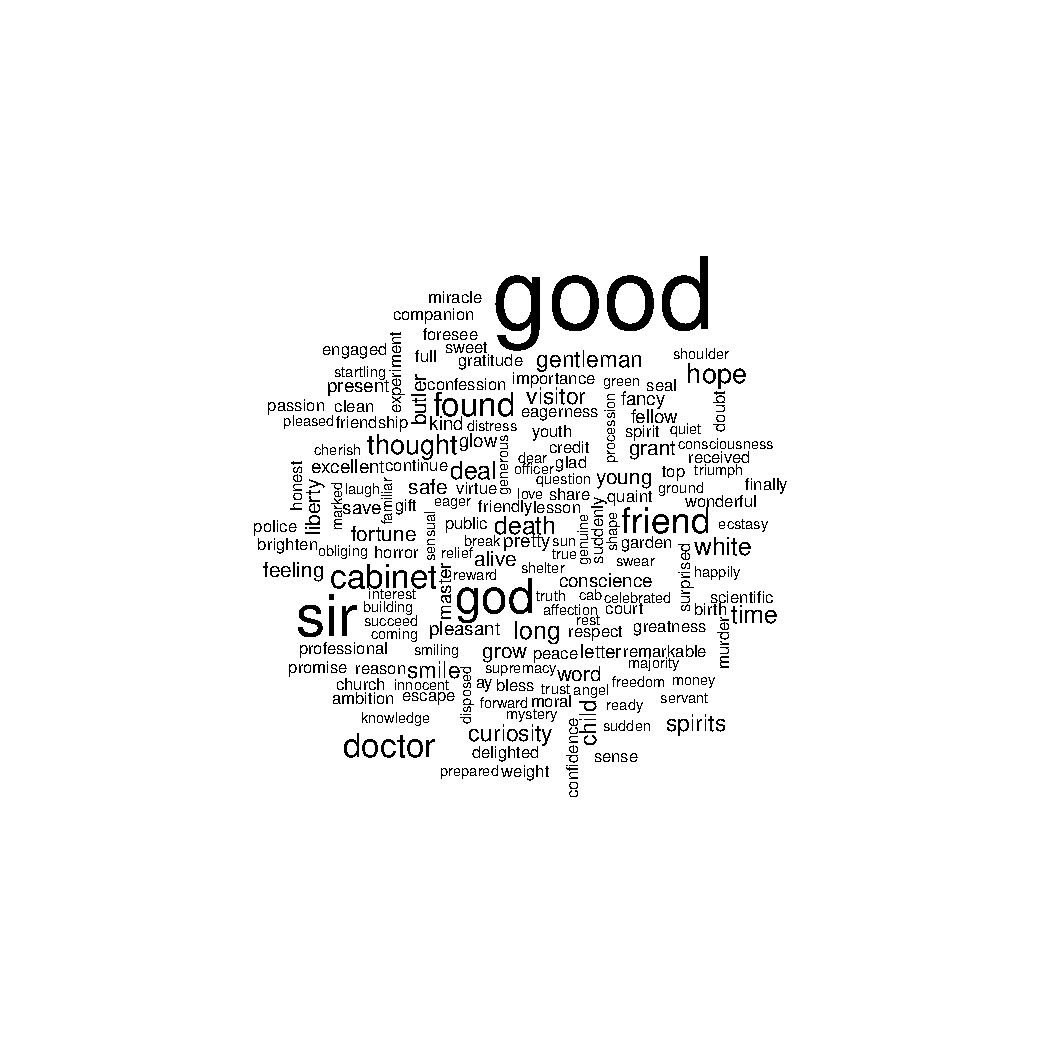
\includegraphics[width=\maxwidth]{figure/unnamed-chunk-8-1} 

\end{knitrout}

\end{document}














